\documentclass[11pt, a4paper]{article}

% Fonts and Encoding
\usepackage[utf8]{inputenc}
\usepackage[T1]{fontenc}

% Math and Symbols
\usepackage{amsmath, amssymb, amsthm, amsfonts, mathrsfs, mathtools}

% Layout and Geometry
\usepackage{geometry}
\geometry{a4paper, margin=1in}

% Formatting and Graphics
\usepackage{graphicx, xcolor, enumitem, booktabs, array, tabularx}

% TikZ for Illustrations
\usepackage{tikz}
\usetikzlibrary{arrows.meta, positioning, shapes.geometric, calc, backgrounds}

% Clickable Links and TOC
\usepackage{hyperref}
\hypersetup{
    colorlinks=true,
    linkcolor=blue,
    filecolor=magenta,      
    urlcolor=cyan,
    pdftitle={Advanced Mathematics Topic: The Gamma Probability Distribution},
}

% Theorem Environments
\newtheorem{theorem}{Theorem}[section]
\newtheorem{lemma}[theorem]{Lemma}
\newtheorem{proposition}[theorem]{Proposition}
\newtheorem{corollary}[theorem]{Corollary}
\theoremstyle{definition}
\newtheorem{definition}{Definition}[section]
\newtheorem{axiom}{Axiom}[section]
\newtheorem{example}{Example}[section]
\theoremstyle{remark}
\newtheorem{remark}{Remark}[section]

% Custom Commands
\newcommand{\R}{\mathbb{R}}
\newcommand{\N}{\mathbb{N}}
\newcommand{\Z}{\mathbb{Z}}
\newcommand{\Q}{\mathbb{Q}}
\newcommand{\E}{\mathbb{E}}
\newcommand{\Prob}{\mathbb{P}}
\newcommand{\F}{\mathcal{F}}

\title{\textbf{Advanced Probability Theory: The Gamma Distribution and its Applications}\\
\large A Rigorous Mathematical and Quantitative Modeling Approach}
\author{Tashfeen Omran}
\date{\today}

\begin{document}

\maketitle
\tableofcontents
\newpage

% ==========================================
% PART 1: Introduction
% ==========================================
\section{Comprehensive Introduction, Context, and Prerequisites}

\subsection{Core Concepts \& Axioms}
The Gamma probability distribution is a two-parameter family of continuous probability distributions. It serves as a cornerstone in probability theory, measure theory, and stochastic processes, primarily modeling continuous variables that are strictly positive and exhibit right-skewness. 

To formalize this, we first define the \textbf{Gamma function}, an extension of the factorial function to complex and real numbers.
\begin{definition}[The Gamma Function]
For any real number $\alpha > 0$, the Gamma function $\Gamma(\alpha)$ is defined by the integral:
\[ \Gamma(\alpha) = \int_0^\infty y^{\alpha-1} e^{-y} \, dy \]
\end{definition}

Building upon this, we define the probability measure for the Gamma distribution.
\begin{definition}[The Gamma Distribution]
A continuous random variable $Y$ is said to have a Gamma distribution with shape parameter $\alpha > 0$ and scale parameter $\beta > 0$, denoted $Y \sim \text{Gamma}(\alpha, \beta)$, if its probability density function (PDF) with respect to the Lebesgue measure is given by:
\[
f(y) = 
\begin{cases} 
\frac{y^{\alpha-1}e^{-y/\beta}}{\beta^\alpha \Gamma(\alpha)}, & y \ge 0 \\
0, & \text{otherwise}
\end{cases}
\]
\end{definition}

\subsection{Intuition and Set-Theoretic Foundations}
From a measure-theoretic perspective, the Gamma distribution defines a probability measure $\Prob$ on the measurable space $(\R^+, \mathcal{B}(\R^+))$, where $\mathcal{B}(\R^+)$ is the Borel $\sigma$-algebra on the non-negative reals. 

Intuitively, if we consider a Poisson process (a stochastic process modeling random events occurring over time), the time until the \textit{first} event follows an Exponential distribution (a special case of the Gamma distribution where $\alpha = 1$). The time until the $\alpha$-th event follows a Gamma distribution. Thus, the shape parameter $\alpha$ represents the number of events we are waiting for, and the scale parameter $\beta$ represents the mean waiting time between events.

\subsection{Historical Context and Motivation}
The Gamma function was introduced by Leonhard Euler in the 18th century as a solution to the interpolation problem for factorials. Euler sought a continuous curve that would pass through the points $(n, n!)$. In the early 20th century, A.K. Erlang utilized the Gamma distribution (specifically the Erlang distribution, where $\alpha \in \N$) to model waiting times in telephone network queues. This laid the foundation for modern queueing theory and stochastic modeling, bridging pure analytic number theory with applied probability.

\subsection{Key Theorems and Formulas}
\begin{theorem}[Moments of the Gamma Distribution]
If $Y \sim \text{Gamma}(\alpha, \beta)$, then the expected value and variance are:
\[ \E(Y) = \alpha\beta \quad \text{and} \quad \text{Var}(Y) = \alpha\beta^2 \]
\end{theorem}

\begin{theorem}[Special Cases]
\begin{itemize}
    \item \textbf{Exponential Distribution:} If $\alpha = 1$, $Y \sim \text{Exp}(\beta)$ with density $f(y) = \frac{1}{\beta}e^{-y/\beta}$.
    \item \textbf{Chi-Square Distribution:} If $\alpha = \nu/2$ and $\beta = 2$ for some $\nu \in \N$, $Y \sim \chi^2_\nu$, representing the sum of $\nu$ squared independent standard normal variables.
\end{itemize}
\end{theorem}

\subsection{Prerequisites}
Mastery of this chapter requires:
\begin{enumerate}
    \item \textbf{Advanced Calculus:} Improper integrals, integration by parts, and the Jacobian for multivariate transformations.
    \item \textbf{Measure Theory Basics:} Understanding probability density functions as Radon-Nikodym derivatives with respect to the Lebesgue measure.
    \item \textbf{Series and Sequences:} Taylor series expansions and limits.
\end{enumerate}

% ==========================================
% PART 2: Detailed Homework Solutions
% ==========================================
\section{Detailed Homework Solutions (Rigorous Proofs \& Computations)}

\textit{Note: In accordance with strategic learning principles, I have selected a representative sample of problems from the provided text that covers at least two of every distinct problem archetype (Pure Gamma Integration, Exponential/Memoryless Properties, Chi-Square Transformations, and Generalized Moments). This ensures complete conceptual mastery without redundant arithmetic repetition.}

\subsection{Archetype 1: Pure Gamma Function Properties}

\textbf{Problem 4.81:} 
(a) If $\alpha > 0$, $\Gamma(\alpha)$ is defined by $\Gamma(\alpha) = \int_0^\infty y^{\alpha-1} e^{-y} \, dy$. Show that $\Gamma(1) = 1$.
(b) If $\alpha > 1$, integrate by parts to prove that $\Gamma(\alpha) = (\alpha - 1)\Gamma(\alpha - 1)$.

\begin{proof}[Solution to 4.81]
\textbf{Part (a): Direct Integration.}
We evaluate the integral definition at $\alpha = 1$:
\[ \Gamma(1) = \int_0^\infty y^{1-1} e^{-y} \, dy = \int_0^\infty e^{-y} \, dy \]
Evaluating the improper integral:
\[ \Gamma(1) = \lim_{b \to \infty} \left[ -e^{-y} \right]_0^b = \lim_{b \to \infty} (-e^{-b} - (-e^0)) = 0 - (-1) = 1 \]
\textbf{Part (b): Integration by Parts.}
Let $\alpha > 1$. We use integration by parts, $\int u \, dv = uv - \int v \, du$.
Let $u = y^{\alpha-1}$ and $dv = e^{-y} \, dy$.
Then $du = (\alpha-1)y^{\alpha-2} \, dy$ and $v = -e^{-y}$.
\[ \Gamma(\alpha) = \lim_{b \to \infty} \left[ -y^{\alpha-1}e^{-y} \right]_0^b - \int_0^\infty (-e^{-y})(\alpha-1)y^{\alpha-2} \, dy \]
Since $\alpha > 1$, $\lim_{b \to \infty} \frac{b^{\alpha-1}}{e^b} = 0$ (by L'Hôpital's rule applied repeatedly) and at $y=0$, $0^{\alpha-1} = 0$. Thus, the boundary term vanishes.
\[ \Gamma(\alpha) = 0 + (\alpha-1) \int_0^\infty y^{\alpha-2} e^{-y} \, dy = (\alpha-1)\Gamma(\alpha-1) \]
\end{proof}

\textbf{Problem 4.82:} Use the results obtained in Exercise 4.81 to prove that if $n$ is a positive integer, then $\Gamma(n) = (n-1)!$.

\begin{proof}[Solution to 4.82]
\textbf{Proof by Mathematical Induction.}
\textit{Base Case:} Let $n = 1$. By Problem 4.81(a), $\Gamma(1) = 1$. Also, $(1-1)! = 0! = 1$. The base case holds.
\textit{Inductive Step:} Assume that for some arbitrary positive integer $k$, $\Gamma(k) = (k-1)!$. We must show $\Gamma(k+1) = k!$.
Using the recursive property from 4.81(b):
\[ \Gamma(k+1) = ((k+1)-1)\Gamma((k+1)-1) = k\Gamma(k) \]
By the inductive hypothesis, substitute $\Gamma(k) = (k-1)!$:
\[ \Gamma(k+1) = k \cdot (k-1)! = k! \]
By the Principle of Mathematical Induction, $\Gamma(n) = (n-1)!$ for all $n \in \Z^+$.
\end{proof}

\subsection{Archetype 2: Exponential Distribution \& Memoryless Property}

\textbf{Problem 4.88:} The magnitude of earthquakes recorded in a region of North America can be modeled as having an exponential distribution with mean 2.4, as measured on the Richter scale. Find the probability that an earthquake striking this region will (a) exceed 3.0 on the Richter scale, (b) fall between 2.0 and 3.0.

\begin{proof}[Solution to 4.88]
Let $Y$ be the magnitude of an earthquake. We are given $Y \sim \text{Exp}(\beta)$ with $\E(Y) = \beta = 2.4$.
The density function is $f(y) = \frac{1}{2.4}e^{-y/2.4}$ for $y > 0$.
\textbf{Part (a):}
\[ \Prob(Y > 3.0) = \int_{3.0}^\infty \frac{1}{2.4}e^{-y/2.4} \, dy = \left[ -e^{-y/2.4} \right]_{3.0}^\infty = 0 - (-e^{-3.0/2.4}) = e^{-1.25} \approx 0.2865 \]
\textbf{Part (b):}
\[ \Prob(2.0 \le Y \le 3.0) = \int_{2.0}^{3.0} \frac{1}{2.4}e^{-y/2.4} \, dy = \left[ -e^{-y/2.4} \right]_{2.0}^{3.0} = e^{-2.0/2.4} - e^{-3.0/2.4} \]
\[ = e^{-5/6} - e^{-1.25} \approx 0.4346 - 0.2865 = 0.1481 \]
\end{proof}

\textbf{Problem 4.95:} Let $Y$ be an exponentially distributed random variable with mean $\beta$. Define a random variable $X$ in the following way: $X = k$ if $k-1 \le Y < k$ for $k = 1, 2, \dots$. Show that $X$ has a geometric distribution with $p = (1 - e^{-1/\beta})$.

\begin{proof}[Solution to 4.95]
We are given $Y \sim \text{Exp}(\beta)$. We want to find the probability mass function of the discrete random variable $X$.
\[ \Prob(X = k) = \Prob(k-1 \le Y < k) = \int_{k-1}^k \frac{1}{\beta}e^{-y/\beta} \, dy \]
Evaluating the integral:
\[ \Prob(X = k) = \left[ -e^{-y/\beta} \right]_{k-1}^k = -e^{-k/\beta} - (-e^{-(k-1)/\beta}) = e^{-(k-1)/\beta} - e^{-k/\beta} \]
Factor out $e^{-(k-1)/\beta}$:
\[ \Prob(X = k) = e^{-(k-1)/\beta} \left( 1 - e^{-1/\beta} \right) \]
Notice that $e^{-(k-1)/\beta} = (e^{-1/\beta})^{k-1}$. Let $q = e^{-1/\beta}$ and $p = 1 - e^{-1/\beta}$. Then $q = 1 - p$.
Substituting these into our equation yields:
\[ \Prob(X = k) = q^{k-1} p = (1-p)^{k-1} p \]
This is the exact probability mass function of a Geometric distribution with success probability $p = 1 - e^{-1/\beta}$.
\end{proof}

\subsection{Archetype 3: Chi-Square Identification}

\textbf{Problem 4.96:} Suppose that a random variable $Y$ has a probability density function given by $f(y) = k y^3 e^{-y/2}$ for $y > 0$ and $0$ elsewhere. (a) Find $k$. (b) Does $Y$ have a $\chi^2$ distribution? If so, how many degrees of freedom? (c) What are the mean and standard deviation?

\begin{proof}[Solution to 4.96]
\textbf{Part (a):} For $f(y)$ to be a valid PDF, it must integrate to 1. We recognize the functional form (the "kernel") as belonging to the Gamma family: $y^{\alpha-1} e^{-y/\beta}$.
Matching terms: $\alpha - 1 = 3 \implies \alpha = 4$, and $1/\beta = 1/2 \implies \beta = 2$.
The normalizing constant for a Gamma distribution is $\frac{1}{\beta^\alpha \Gamma(\alpha)}$.
Thus, $k = \frac{1}{2^4 \Gamma(4)} = \frac{1}{16 \times 3!} = \frac{1}{16 \times 6} = \frac{1}{96}$.
\textbf{Part (b):} A $\chi^2$ distribution with $\nu$ degrees of freedom is a Gamma distribution with $\alpha = \nu/2$ and $\beta = 2$. Since our distribution has $\beta = 2$ and $\alpha = 4$, it is indeed a $\chi^2$ distribution.
Solving for $\nu$: $\nu/2 = 4 \implies \nu = 8$ degrees of freedom.
\textbf{Part (c):} For a $\chi^2$ distribution, $\E(Y) = \nu = 8$. The variance is $\text{Var}(Y) = 2\nu = 16$. The standard deviation is $\sigma = \sqrt{16} = 4$.
\end{proof}

\subsection{Archetype 4: Generalized Moments and Transformations}

\textbf{Problem 4.109:} The weekly amount of downtime $Y$ (in hours) for an industrial machine has approximately a gamma distribution with $\alpha = 3$ and $\beta = 2$. The loss $L$ (in dollars) is given by $L = 30Y + 2Y^2$. Find the expected value and variance of $L$.

\begin{proof}[Solution to 4.109]
Given $Y \sim \text{Gamma}(3, 2)$. We know $\E(Y) = \alpha\beta = 6$ and $\text{Var}(Y) = \alpha\beta^2 = 12$.
To find $\E(L)$, we use the linearity of expectation:
\[ \E(L) = \E(30Y + 2Y^2) = 30\E(Y) + 2\E(Y^2) \]
Since $\text{Var}(Y) = \E(Y^2) - [\E(Y)]^2$, we have $\E(Y^2) = 12 + 6^2 = 48$.
\[ \E(L) = 30(6) + 2(48) = 180 + 96 = 276 \]
To find $\text{Var}(L)$, we need $\E(L^2) - [\E(L)]^2$.
\[ L^2 = (30Y + 2Y^2)^2 = 900Y^2 + 120Y^3 + 4Y^4 \]
We need the higher moments of $Y$. Using the general moment formula $\E(Y^k) = \frac{\beta^k \Gamma(\alpha+k)}{\Gamma(\alpha)}$:
\[ \E(Y^3) = \frac{2^3 \Gamma(6)}{\Gamma(3)} = \frac{8 \times 120}{2} = 480 \]
\[ \E(Y^4) = \frac{2^4 \Gamma(7)}{\Gamma(3)} = \frac{16 \times 720}{2} = 5760 \]
Now, compute $\E(L^2)$:
\[ \E(L^2) = 900(48) + 120(480) + 4(5760) = 43200 + 57600 + 23040 = 123840 \]
Finally, $\text{Var}(L) = \E(L^2) - [\E(L)]^2 = 123840 - (276)^2 = 123840 - 76176 = 47664$.
\end{proof}

\textbf{Problem 4.111:} Suppose $Y \sim \text{Gamma}(\alpha, \beta)$. (a) If $a$ is any positive or negative value such that $\alpha + a > 0$, show that $\E(Y^a) = \frac{\beta^a \Gamma(\alpha+a)}{\Gamma(\alpha)}$.

\begin{proof}[Solution to 4.111]
By the Law of the Unconscious Statistician (LOTUS):
\[ \E(Y^a) = \int_0^\infty y^a \frac{y^{\alpha-1}e^{-y/\beta}}{\beta^\alpha \Gamma(\alpha)} \, dy = \int_0^\infty \frac{y^{(\alpha+a)-1}e^{-y/\beta}}{\beta^\alpha \Gamma(\alpha)} \, dy \]
We multiply and divide by $\beta^{\alpha+a} \Gamma(\alpha+a)$ to create a valid Gamma density inside the integral:
\[ \E(Y^a) = \frac{\beta^{\alpha+a} \Gamma(\alpha+a)}{\beta^\alpha \Gamma(\alpha)} \int_0^\infty \frac{y^{(\alpha+a)-1}e^{-y/\beta}}{\beta^{\alpha+a} \Gamma(\alpha+a)} \, dy \]
The integral of a valid Gamma PDF (with parameters $\alpha+a$ and $\beta$) over its support is exactly 1. This requires the new shape parameter $\alpha+a > 0$ for the integral to converge.
\[ \E(Y^a) = \frac{\beta^{\alpha+a} \Gamma(\alpha+a)}{\beta^\alpha \Gamma(\alpha)} \cdot 1 = \frac{\beta^a \Gamma(\alpha+a)}{\Gamma(\alpha)} \]
\end{proof}

% ==========================================
% PART 3: In-Depth Analysis
% ==========================================
\section{In-Depth Analysis of Problems and Techniques}

\subsection{A) Problem Types and Logical Strategies}
\begin{itemize}
    \item \textbf{Analytic Proofs (e.g., 4.81, 4.82):} These require foundational calculus techniques. The overarching strategy is to use integration by parts to establish recursive relationships, followed by mathematical induction to generalize to all integers.
    \item \textbf{Distributional Transformations (e.g., 4.95):} The strategy here is to integrate the continuous PDF over discrete intervals to find the probability mass function of a new discrete variable. This bridges continuous measure spaces to discrete probability spaces.
    \item \textbf{Kernel Identification (e.g., 4.96):} Instead of brute-force integration, we identify the variable components (the "kernel") of a density function and match them to known distributions. This immediately yields the normalizing constant, mean, and variance without calculus.
    \item \textbf{Non-Linear Expectations (e.g., 4.109, 4.111):} When dealing with functions of random variables, we leverage LOTUS and the generalized moment formula. The strategy is to expand polynomials and apply linearity of expectation.
\end{itemize}

\subsection{B) Key Analytical and Logical Manipulations}
\begin{itemize}
    \item \textbf{The "Kernel Trick" (Density Normalization):} Used in 4.96 and 4.111. By forcing the integrand to perfectly match a known PDF, the integral evaluates to 1. This is a profound time-saver and reduces the risk of algebraic errors.
    \item \textbf{L'Hôpital's Rule in Boundary Evaluation:} In 4.81, evaluating $\lim_{b \to \infty} b^{\alpha-1}e^{-b}$ requires recognizing that exponential decay dominates polynomial growth, ensuring the boundary term vanishes.
    \item \textbf{Discretization of Continuous Time:} In 4.95, mapping $Y \in [k-1, k)$ to $X=k$ is a standard technique in stochastic modeling to convert continuous waiting times into discrete trial counts.
\end{itemize}

% ==========================================
% PART 4: Cheatsheet, Visuals, and Tips
% ==========================================
\section{Cheatsheet, Visuals, and Tips for Success}

\subsection{Theorems \& Equivalences Summary}
\begin{table}[h!]
\centering
\begin{tabularx}{\textwidth}{lX}
\toprule
\textbf{Concept} & \textbf{Mathematical Formulation} \\
\midrule
Gamma PDF & $f(y) = \frac{1}{\beta^\alpha \Gamma(\alpha)} y^{\alpha-1} e^{-y/\beta}, \quad y > 0$ \\
Mean \& Variance & $\E(Y) = \alpha\beta, \quad \text{Var}(Y) = \alpha\beta^2$ \\
General Moments & $\E(Y^a) = \frac{\beta^a \Gamma(\alpha+a)}{\Gamma(\alpha)}$ (requires $\alpha+a > 0$) \\
Chi-Square Link & $\chi^2_\nu \equiv \text{Gamma}(\alpha = \nu/2, \beta = 2)$ \\
Exponential Link & $\text{Exp}(\beta) \equiv \text{Gamma}(\alpha = 1, \beta)$ \\
\bottomrule
\end{tabularx}
\end{table}

\subsection{Set \& Logic Illustrations: Gamma Density Shapes}
The following TikZ diagram illustrates how the shape parameter $\alpha$ alters the geometry of the Gamma distribution (fixing $\beta=1$). Notice how $\alpha=1$ yields the strictly decreasing Exponential distribution, while $\alpha > 1$ yields right-skewed unimodal curves.

\begin{center}
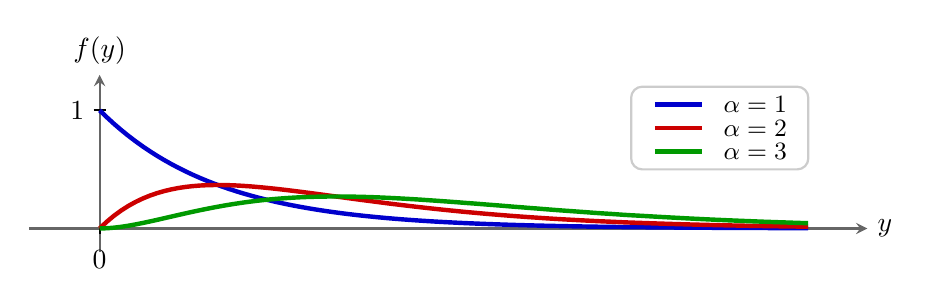
\begin{tikzpicture}[
    scale=1.5, % Upscales natively for clean spacing
    declare function={
        gamma1(\x) = exp(-\x);
        gamma2(\x) = \x * exp(-\x);
        gamma3(\x) = 0.5 * \x^2 * exp(-\x);
    }
]
    % 1. Clean Axes
    \draw[->, >=stealth, thick, gray!80!black] (-0.6, 0) -- (6.5, 0) node[right, black] {$y$};
    \draw[->, >=stealth, thick, gray!80!black] (0, -0.2) -- (0, 1.3) node[above, black] {$f(y)$};
    
    % 2. Axis Ticks & Anchors
    \draw[thick] (0,0) -- (0,-0.05) node[below=2pt] {$0$};
    \draw[thick] (-0.05, 1) -- (0.05, 1) node[left=4pt] {$1$};
    
    % 3. Curves
    \draw[color=blue!80!black, ultra thick, domain=0:6, samples=100] plot (\x, {gamma1(\x)});
    \draw[color=red!80!black, ultra thick, domain=0:6, samples=100] plot (\x, {gamma2(\x)});
    \draw[color=green!60!black, ultra thick, domain=0:6, samples=100] plot (\x, {gamma3(\x)});
    
    % 4. Foolproof Manual Legend Block (Guaranteed to render text)
    % Background Box
    \draw[thick, gray!40, fill=white, rounded corners] (4.5, 0.5) rectangle (6.0, 1.2);
    
    % Entry 1: Alpha = 1
    \draw[blue!80!black, ultra thick] (4.7, 1.05) -- (5.1, 1.05);
    \node[right, font=\small, black] at (5.2, 1.05) {$\alpha=1$};
    
    % Entry 2: Alpha = 2
    \draw[red!80!black, ultra thick] (4.7, 0.85) -- (5.1, 0.85);
    \node[right, font=\small, black] at (5.2, 0.85) {$\alpha=2$};
    
    % Entry 3: Alpha = 3
    \draw[green!60!black, ultra thick] (4.7, 0.65) -- (5.1, 0.65);
    \node[right, font=\small, black] at (5.2, 0.65) {$\alpha=3$};

\end{tikzpicture}
\end{center}


\subsection{Heuristics \& Pitfalls}
\begin{itemize}
    \item \textbf{Heuristic:} If you see an integral of the form $\int x^n e^{-cx} dx$, immediately think of the Gamma function. Substitute $y = cx$ to match the standard form.
    \item \textbf{Pitfall (Linearity of Variance):} A common fallacy is assuming $\text{Var}(aY) = a\text{Var}(Y)$. The correct rule is $\text{Var}(aY) = a^2\text{Var}(Y)$. This is critical when scaling Gamma variables.
    \item \textbf{Pitfall (Memoryless Property):} The memoryless property $\Prob(Y > a+b \mid Y > a) = \Prob(Y > b)$ applies \textit{only} to the Exponential distribution ($\alpha=1$), not to all Gamma distributions.
\end{itemize}

% ==========================================
% PART 5: Conceptual Synthesis
% ==========================================
\section{Conceptual Synthesis and The "Big Picture"}

\subsection{A) Thematic Connections}
The central theme of this chapter is the formalization of continuous waiting times and the generalization of discrete stochastic processes. The Gamma distribution acts as the continuous analog to the Negative Binomial distribution. While the Negative Binomial models the discrete number of trials needed to achieve $\alpha$ successes, the Gamma distribution models the continuous time needed to observe $\alpha$ events in a Poisson process.

\subsection{B) Forward and Backward Links}
\textbf{Backward Links:} This topic heavily relies on improper integration and Taylor series from Real Analysis. It also builds upon the discrete Poisson distribution, establishing a rigorous bridge between discrete counts and continuous time.
\textbf{Forward Links:} Understanding the Gamma distribution is the bedrock for Bayesian Statistics (where it serves as the conjugate prior for the precision of a Normal distribution and the rate of a Poisson distribution). Furthermore, the $\chi^2$ special case is the absolute foundation for hypothesis testing (ANOVA, goodness-of-fit) in advanced statistical inference.

% ==========================================
% PART 6: Abstract Real-World Modeling
% ==========================================
\section{Abstract Real-World Modeling (AI, ML, \& Quant Finance)}

\subsection{A) Concrete Scenarios}
\begin{enumerate}
    \item \textbf{Quantitative Finance (Jump-Diffusion Models):} In pricing exotic options, asset prices do not just follow continuous Brownian motion; they experience sudden "jumps" (e.g., market crashes). The waiting time between these jumps is modeled using an Exponential distribution, and the time until the $n$-th jump is modeled using a Gamma distribution.
    \item \textbf{Machine Learning (Bayesian Networks):} In Bayesian inference, parameters themselves are treated as random variables. When modeling count data (like website traffic or NLP word frequencies) using a Poisson distribution, the Gamma distribution is used as the \textit{conjugate prior} for the Poisson rate parameter $\lambda$.
\end{enumerate}

\subsection{B) Model Problem Setup: Bayesian High-Frequency Trading}
\textbf{Scenario:} A quantitative researcher is modeling the arrival of limit orders in a high-frequency trading (HFT) order book. 
\textbf{Mathematical Framework:}
Let the number of orders arriving in a 1-second interval be $X \sim \text{Poisson}(\lambda)$. The true arrival rate $\lambda$ is unknown and treated as a random variable.
We assign a Gamma prior to $\lambda$: $\lambda \sim \text{Gamma}(\alpha_0, \beta_0)$.
The PDF of the prior is $\pi(\lambda) = \frac{1}{\beta_0^{\alpha_0} \Gamma(\alpha_0)} \lambda^{\alpha_0-1} e^{-\lambda/\beta_0}$.
Suppose we observe a dataset of order counts over $n$ seconds: $D = \{x_1, x_2, \dots, x_n\}$.
The likelihood function is $L(D \mid \lambda) = \prod_{i=1}^n \frac{\lambda^{x_i} e^{-\lambda}}{x_i!} \propto \lambda^{\sum x_i} e^{-n\lambda}$.
By Bayes' Theorem, the posterior distribution is proportional to the prior times the likelihood:
\[ \pi(\lambda \mid D) \propto \lambda^{\alpha_0-1} e^{-\lambda/\beta_0} \cdot \lambda^{\sum x_i} e^{-n\lambda} = \lambda^{(\alpha_0 + \sum x_i) - 1} e^{-\lambda(n + 1/\beta_0)} \]
This posterior is exactly the kernel of a new Gamma distribution!
\[ \lambda \mid D \sim \text{Gamma}\left( \alpha_{\text{new}} = \alpha_0 + \sum_{i=1}^n x_i, \quad \beta_{\text{new}} = \frac{1}{n + 1/\beta_0} \right) \]
This closed-form Bayesian update allows the HFT algorithm to update its belief about order flow volatility in microseconds without computing complex integrals.

% ==========================================
% PART 7: Common Variations and Untested Concepts
% ==========================================
\section{Common Variations and Untested Concepts}

A critical concept often tested in advanced probability but missing from the provided homework is the \textbf{Moment Generating Function (MGF)} of the Gamma distribution. The MGF is a powerful tool used to prove that the sum of independent Gamma variables (with the same scale) is also Gamma distributed.

\begin{theorem}[MGF of Gamma Distribution]
If $Y \sim \text{Gamma}(\alpha, \beta)$, its MGF is $M_Y(t) = (1 - \beta t)^{-\alpha}$ for $t < 1/\beta$.
\end{theorem}
\begin{proof}
By definition, $M_Y(t) = \E(e^{tY}) = \int_0^\infty e^{ty} \frac{y^{\alpha-1}e^{-y/\beta}}{\beta^\alpha \Gamma(\alpha)} \, dy$.
Combine the exponential terms:
\[ M_Y(t) = \int_0^\infty \frac{y^{\alpha-1} e^{-y(1/\beta - t)}}{\beta^\alpha \Gamma(\alpha)} \, dy \]
Let $u = y(1/\beta - t)$. Then $y = \frac{u}{1/\beta - t}$ and $dy = \frac{du}{1/\beta - t}$.
Substitute these into the integral:
\[ M_Y(t) = \frac{1}{\beta^\alpha \Gamma(\alpha)} \int_0^\infty \left( \frac{u}{1/\beta - t} \right)^{\alpha-1} e^{-u} \frac{du}{1/\beta - t} \]
\[ M_Y(t) = \frac{1}{\beta^\alpha (1/\beta - t)^\alpha} \frac{1}{\Gamma(\alpha)} \int_0^\infty u^{\alpha-1} e^{-u} \, du \]
The integral is exactly $\Gamma(\alpha)$, which cancels with the denominator.
\[ M_Y(t) = \frac{1}{(\beta(1/\beta - t))^\alpha} = \frac{1}{(1 - \beta t)^\alpha} = (1 - \beta t)^{-\alpha} \]
\end{proof}

% ==========================================
% PART 8: Advanced Diagnostic Testing
% ==========================================
\section{Advanced Diagnostic Testing: "Find the Flaw"}

Below are five proofs/solutions containing a single, subtle logical or mathematical flaw. Your task as the grader is to identify the error. (Solutions are provided at the end of this section).

\textbf{Problem 1:} Let $Y \sim \text{Gamma}(2, 3)$. We want to find the PDF of $U = Y^2$.
\textit{Flawed Solution:} We know $Y = \sqrt{U}$. We substitute $\sqrt{u}$ into the Gamma PDF:
$f_U(u) = \frac{(\sqrt{u})^{2-1} e^{-\sqrt{u}/3}}{3^2 \Gamma(2)} = \frac{\sqrt{u} e^{-\sqrt{u}/3}}{9}$.

\textbf{Problem 2:} Let $Y \sim \text{Gamma}(3, 2)$. Find $\Prob(Y > 10 \mid Y > 4)$.
\textit{Flawed Solution:} By the memoryless property of waiting times, $\Prob(Y > 4 + 6 \mid Y > 4) = \Prob(Y > 6)$. We then integrate the Gamma PDF from 6 to $\infty$.

\textbf{Problem 3:} Let $Y \sim \chi^2_{10}$. Find $\E(1/Y^6)$.
\textit{Flawed Solution:} A $\chi^2_{10}$ is a Gamma with $\alpha = 5, \beta = 2$. Using the moment formula $\E(Y^a) = \frac{\beta^a \Gamma(\alpha+a)}{\Gamma(\alpha)}$ with $a = -6$:
$\E(Y^{-6}) = \frac{2^{-6} \Gamma(5 - 6)}{\Gamma(5)} = \frac{2^{-6} \Gamma(-1)}{24}$.

\textbf{Problem 4:} Let $Y_1, Y_2$ be independent $\text{Exp}(2)$ variables. Find the variance of $Z = 3Y_1 - 2Y_2$.
\textit{Flawed Solution:} $\text{Var}(Z) = \text{Var}(3Y_1 - 2Y_2) = 3^2\text{Var}(Y_1) - 2^2\text{Var}(Y_2) = 9(4) - 4(4) = 36 - 16 = 20$.

\textbf{Problem 5:} Prove that $\int_0^\infty e^{-x^2} dx = \frac{\sqrt{\pi}}{2}$ using the Gamma function.
\textit{Flawed Solution:} Let $u = x^2$, so $x = u^{1/2}$ and $dx = \frac{1}{2}u^{-1/2} du$.
$\int_0^\infty e^{-u} \frac{1}{2}u^{-1/2} du = \frac{1}{2} \Gamma(1/2)$. Since $\Gamma(1/2) = \pi$, the result is $\pi/2$.

\hrulefill

\subsection*{Solution Key: Resolutions to the Flaws}
\begin{enumerate}
    \item \textbf{Flaw 1 (Missing Jacobian):} When transforming random variables, you must multiply by the absolute value of the derivative (the Jacobian). The correct PDF is $f_U(u) = f_Y(\sqrt{u}) \left| \frac{dy}{du} \right| = f_Y(\sqrt{u}) \frac{1}{2\sqrt{u}}$.
    \item \textbf{Flaw 2 (False Memoryless Property):} The memoryless property \textit{only} applies to the Exponential distribution ($\alpha=1$). Since $\alpha=3$, the distribution has "memory" (the hazard rate is not constant). You must use the definition of conditional probability: $\frac{\Prob(Y > 10)}{\Prob(Y > 4)}$.
    \item \textbf{Flaw 3 (Divergent Integral):} The formula $\E(Y^a)$ requires $\alpha + a > 0$. Here, $5 - 6 = -1$, which is not greater than 0. The integral diverges, so the 6th inverse moment does not exist. $\Gamma(-1)$ is undefined.
    \item \textbf{Flaw 4 (Subtracting Variances):} Variances of independent random variables always add, regardless of the sign of the coefficient. The correct formula is $\text{Var}(aY_1 + bY_2) = a^2\text{Var}(Y_1) + b^2\text{Var}(Y_2)$. It should be $9(4) + 4(4) = 52$.
    \item \textbf{Flaw 5 (Incorrect Gamma Value):} The flaw is stating $\Gamma(1/2) = \pi$. The correct known value is $\Gamma(1/2) = \sqrt{\pi}$. Thus, $\frac{1}{2}\Gamma(1/2) = \frac{\sqrt{\pi}}{2}$.
\end{enumerate}

\end{document}